\documentclass{beamer}
\usepackage[utf8]{inputenc}
\usepackage[ngerman]{babel}

\usetheme[deutsch]{KIT}
\author{Simon Bischof (simon.bischof2@student.kit.edu)}
\title{Tutorium Theoretische Grundlagen der Informatik}
\subtitle{Simon Bischof}
\institute{Institut f\"{u}r Kryptographie und Sicherheit}
\TitleImage[scale=0.7]{tmaschine.png}

\newcommand{\F}{\Sigma^*}
\newcommand{\N}{\ensuremath \mathbb{N}}
\newcommand{\R}{\ensuremath \mathbb{R}}
\renewcommand{\P}{\ensuremath \mathcal{P}}
\newcommand{\NP}{\ensuremath \mathcal{NP}}
\newcommand{\NPC}{\ensuremath \mathcal{NP-C}}

\begin{document}
\shorthandoff{"}
\begin{frame}
\maketitle
\end{frame}

\begin{frame}
\frametitle{\LARGE Geh wählen!}
Nächste Woche:
\begin{itemize}
\item Wahl des Studierendenparlaments
\item Fachschaftssprecher-Wahl
\item Wahl der Frauenreferentin (nur für Frauen)
\item Wahl des Ausländerreferenten (nur für Studenten mit anderer Staatsangehörigkeit)
\item Urabstimmung über die Satzung der Verfassten Studierendenschaft
\end{itemize}
\end{frame}

\begin{frame}
\frametitle{Zur Kolmogorov-Komplexität}
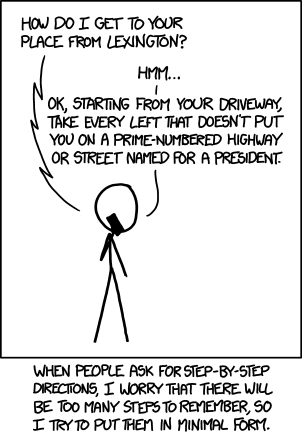
\includegraphics[scale=0.35]{kolmogorov_directions.png}\\
{\tiny Quelle: xkcd.com/1155}
\end{frame}

\begin{frame}
\frametitle{Wie beweise ich $L\in\NPC$?}
\begin{itemize}
\item $L\in\NP$
\item $B\leq_p L$ für ein $B\in\NPC$\pause
\item und nun? Wie bekommen wir ein erstes $\NPC$-Problem?\pause
\item Satz von Cook: SAT$\in\NPC$ (SAT in KNF)
\end{itemize}
\end{frame}

\begin{frame}
\frametitle{Probleme aus $\NPC$, wichtige Reduktionen}
\begin{itemize}
\item SAT $\leq$ 3SAT\pause
\item 3SAT $\leq$ 3COLOR\pause
\item VERTEX COVER: Geg.: ungerichteter Graph $G=(V,E)$ und $k\in\N$\\
Frage: $\exists V^\prime\subseteq V$ mit $|V^\prime|\leq k$ und $\forall e\in E:e\cap V^\prime\neq\emptyset$?\\ 3SAT $\leq$ VERTEX COVER\pause
\item SUBSET SUM: Gegeben $X\subseteq\N$ endlich, $k\in\N$. $\exists T\subseteq X:\sum\limits_{t\in T}t=k$?\pause
\item HAMILTONIAN PATH $\leq$ HAMILTONIAN CYCLE
\end{itemize}
\end{frame}

\begin{frame}
\frametitle{zum Schluss}
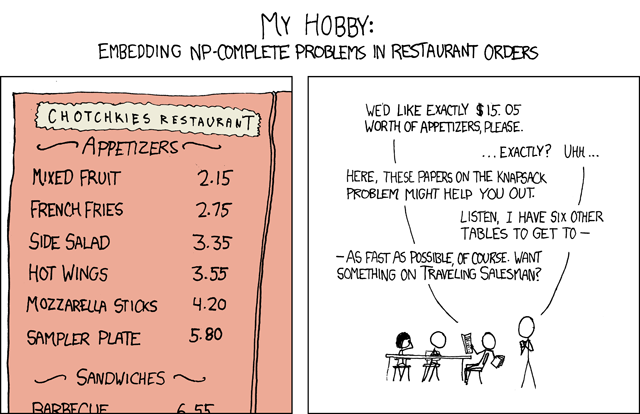
\includegraphics[scale=4]{np_complete.png}\\
{\tiny Quelle: xkcd.com/287}
\end{frame}
\end{document}